\subsection*{Monte Carlo Sampling}

% Week 8

\begin{defe}[Empirical distribution] \label{defe: em_dist}
    Let $x_1 , \ldots , x_n$ be an iid real-valued sample from a cdf $F$. The function
    \begin{equation*}
        F_{n} (x) = \frac{1}{N} \sum_{i=1}^{N} \Id_{\left\{ x_i \leq x \right\}} (x) , \quad x \in \RR
    \end{equation*}
    is called the {\bf empirical cdf} of the data \cite{KroeseDirkP2013SMaC}*{page 196}.
\end{defe}

\begin{figure}[ht]
    \centering
    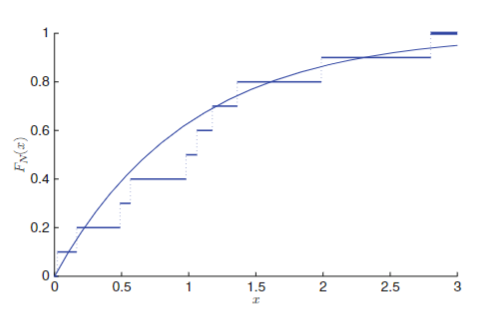
\includegraphics[scale=1.0]{img/bay_inf/emp_cdf_exp_1.png}
    \caption{The empirical cdf \ref{defe: em_dist} for a sample size $10$ from a $\Exp (0.2)$ distribution as well as the true cdf. Image from \cite{KroeseDirkP2013SMaC}*{page 197}.}
    \label{fig: emp_cdf_exp_1}
\end{figure}

Note that for the ordered sample $x_{(1)} < x_{(2)} < \cdots < x_{(N)}$,

\begin{equation*}
    F_{N} \left( x_{(i)} \right) = \frac{i}{N}.
\end{equation*}

assuming for the sake of simplicity that all $\left\{ x_i \right\}$ take on different values. If instead of deterministic $\left\{ x_i \right\}$ we take random $X_i$, then $F_N (x)$ becomes random as well. To distinguish between the deterministic and the random case, let us denote the random empirical cdf by $\hat{F}_{N} (x)$. We now have
\begin{equation*}
    \PP \left[ \hat{F}_{N} (x) = \frac{i}{N} \right] = \PP \left[ X_{(i)} \leq x , X_{(i+1)}  > x \right] = \binom{N}{i} \left( F(x) \right)^{i} \left( 1 - F(x) \right)^{N-i}
\end{equation*}
\cite{KroeseDirkP2013SMaC}*{page 198}. The above equation can be summarized as $N \hat{F}_{N} (x) \sim \Bin (N, F(x))$. Consequently,
\begin{align*}
    \EE \left[ \hat{F}_{N} (x) \right]  & = F(x)                          \\
    \Var \left[ \hat{F}_{N} (x) \right] & = F(x) \left( 1 - F(x) \right).
\end{align*}
Moreover, by the law of large numbers and the central limit theorem, we have
\begin{equation*}
    \PP \left[ \lim_{N \to \infty} \hat{F}_{N} (x) = F (x) \right] = 1,
\end{equation*}
and
\begin{equation*}
    \lim_{N \to \infty} \PP \left[ \frac{\hat{F}_{N} (x) - F(x)}{\sqrt{F(x)(1-F(x)/N)}} \right] = \Phi (z).
\end{equation*}

\begin{defe}[Confidence Intervals] \label{defe: confd_int}
    Let $X_1 , \ldots , X_n$ be random variables with a joint distribution depdending on a parameter $\theta \in \Theta$. Let $T_1 < T_2$ be functions of the data but not of $\theta$. The random interval $(T_1 , T_2)$ is called a {\bf stochastic confidence interval} for $\theta$ with confidence $1 - \alpha$ if
    \begin{equation*}
        \PP_{\theta} \left[ T_1 < \theta < T_2 \right] \geq 1 - \alpha \quad \text{for all} \quad \theta \in \Theta.
    \end{equation*}
    If $t_1$ and $t_2$ are the observed values of $T_1$ and $T_2$, then the interval $(t_1 , t_2)$ is called the {\bf numerical confidence interval} for $\theta$ with confidence $1 - \alpha$ \cite{KroeseDirkP2013SMaC}*{page 128}.
\end{defe}

An approximate $1 - \alpha$ confidence interval for $F(x)$ is
\begin{equation*}
    F_N (x) \pm z_{1 - \alpha / 2} \sqrt{\frac{F_N (x) (1 - F_N (x))}{N}}
\end{equation*}
where $z_{1 - \alpha / 2}$ is the $1 - \alpha / 2$ quantile of the standard normal distribution. Moreover for the ordered sample $x_{(1)} < x_{(2)} < \cdots < x_{(N)}$, an approximate $1 - \alpha$ confidence interval for $F(x_{(i)})$ is
\begin{equation*}
    \frac{i}{N} \pm z_{1 - \alpha / 2} \sqrt{\frac{i(1 - i/n)}{N^2}}
\end{equation*}
\cite{KroeseDirkP2013SMaC}*{page 198}.

\subsubsection*{Simultaneous Confidence Bands}

% Week Lec 2, Ch 7.1

\begin{defe}[Kolmogorov–Smirnov statistic] \label{defe: TBD}
    For a continuous $F$, the statistic of
    \begin{equation*}
        D_n = \sup_{x \in \RR} \left| \hat{F}_N (x) - F(x) \right|
    \end{equation*}
    is called the {\bf Kolmogorov–Smirnov statistic} \cite{KroeseDirkP2013SMaC}*{page 200}.
\end{defe}

Note that this statistic does not depend on $F$ and can be used to test whether iid samples $X_1 , \ldots , X_n$ come from a specified distribution as well as constructing a simultaneous confidence band for $F$. The empirical cdf can be used to estimate any cdf, both discrete and continuous, but it is always 'jumpy' which may be undesirable, for example when the underlying distribution is continuous. When we have continuous data, we may want a continuous density estimate instead. This leads to our next topic of density estimation.

\subsubsection*{Kernel Density Estimation}

\begin{defe}[Kernel Density Estimator] \label{defe: KDE}
    Let $X_1 , \ldots X_n \iid f$ from a continuous distribution with cdf $F$. A {\bf Kernel density estimator} (KDE), also known as a sliding window estimator, with bandwidth $h$ is given by
    \begin{equation*}
        \hat{f} (x;h) = \frac{1}{N} \sum_{i=1}^{N} K \left( \frac{x_i - x}{h} \right).
    \end{equation*}
    The function $K (\cdot)$ is the kernel function ("window shape") and $h$ is the window ("window size").
\end{defe}

There are many choice of $K$, but we shall just focus on the Gaussian kernel.

\begin{defe}[Gaussian Kernel] \label{defe: gauss_kern}
    The {\bf Gaussian Kernel} uses a kernel of
    \begin{equation*}
        K(x) = \frac{1}{\sqrt{2 \pi}} \exp \left( - \frac{1}{2} x^2 \right)
    \end{equation*}
    so that
    \begin{equation*}
        \hat{f} (x;h) = \frac{1}{N} \sum_{i=1}^{N} \frac{1}{\sqrt{2 \pi}} \exp \left( - \frac{1}{2} \left( \frac{x_i - x}{h} \right)^2 \right)
    \end{equation*}
    \cite{KroeseDirkP2013SMaC}*{page 201}.
\end{defe}
% Week 9 content
Essentially, the Gaussian kernel is just an equally weighted $\frac{1}{N}$ normal mixture model. It has $N$ Gaussian "humps", centered at each observation and has standard deviation $h$. As it turns out, the choice of the kernel is not that crucial, but the choice of the bandwidth is very important. An often used {\it rule of thumb} is to take
\begin{equation*}
    h_{\text{Rot}} = \left( \frac{4S^5}{3N} \right)^{4/5}
\end{equation*}
called the Silverman's rule of thumb where $S^2$ is the variance. This is based on a theoretical analysis of the discrepancy between $f_n (x;h)$ and the true pdf, as $n \to \infty$. This rule of thumb is best suited when the underlying data is roughly normal-looking (i.e unimodel and symmeteric). A more recent bandwidth selection methods \cite{10.1214/10-AOS799}, called the theta KDE, adaptively changes the bandwidth.

\subsubsection*{Bootstrap Method}

A key concept in statistics is the idea of a sampling distribution (i.e. the distribution of the sample quantity, if we could repeat the random experiment over and over again). Unfortunately, we typically only get one realization of the random process, from which we compute sample quantity we want (for example the sample mean or medium). So, how can we get a feel about the sampling distribution if we have only one realization?

\begin{exam}[Bootstrap Median] \label{exam: bootstrap_median}
    Suppose we have the following sample
    \begin{equation*}
        6.45 , 3.52 , 3.92 , 0.64 , 3.73 , 2.00, 2.73 , 4.20, 20.58, 6.80, 3.22, 7.11, 1.08 , 5.94.
    \end{equation*}
    From this data, how do we construct a confidence interval for the true population medium $M$ of the distribution $F$ that generated the data? Ideally we sample from $F$ over and over again and each time we compute the sample medium and then we look at the distribution of the computed sample medians. Since we don't have access to the distribution $F$, we can instead employ the bootstrap method.
    \begin{itemize}
        \item To start we take iid sample of size $n$, $x^{\ast}$, from the empirical cdf $F_n$ with replacement.
        \item For each sample, we compute the sample medium $m^{\ast}$ of the resampled data.
        \item Then we look at the $2.5$ percentile and the $97.5$ percentile of the resampled values of the mediums.
        \item This percentiles together provide an approximate $95$ percent confidence interval for the population median $M$.
    \end{itemize}
\end{exam}

We can use the bootstrap method to estimate any property of the sample distribution, for example, the variance of the sample mean, medium or IQR. In general we may be interested in some property $h$ (eg. bias, variance, MSE) of some statistic $H(\bm{x})$ (eg. median, $\frac{1}{\overline{X}}$) we can apply the bootstrap resampling approach to estimate these properties.

    {\centering
        \begin{minipage}{.85\linewidth}
            \begin{algorithm}[H]
                \caption{Bootstrap Method}
                \label{alg: bootstrap}
                \SetAlgoLined
                \DontPrintSemicolon
                \SetKwInOut{Input}{input}\SetKwInOut{Output}{output}

                \Input{Observations $\bm{x}$.}
                \Output{Estimate of $\EE \left[ h(H(\bm{x})) \right]$.}
                \BlankLine
                \For{$i\gets 1 , \ldots , K$}{
                Resample data $\bm{x}_1^{\ast} , \bm{x}_2^{\ast}, \ldots , \bm{x}_n^{\ast}$ from the original data.\;
                For each sample, calculate $h(H_k^{\ast}) = h(H(\bm{x}_k^{\ast}))$\;
                }
                Estimate $\EE \left[ h(H(\bm{x})) \right]$ using $\frac{1}{K} \sum_{i=1}^{K} h(H_k^{\ast})$
                \BlankLine
            \end{algorithm}
        \end{minipage}
        \par
    }

For example to compute the variance of the sample medium we can compute
\begin{equation*}
    \VV (\text{medium}) = \EE \left[ (m - \EE(m)) \right]^2 \simeq \sum_{i=1}^{K} (m_i^{\ast} - \overline{m}^{\ast})^2
\end{equation*}
where $m_i^{\ast}$ is the sample median of the ith resampled dataset and $\overline{m}^{\ast}$ is the mean of the resampled median values. If we replace $F$ by the empirical cdf, $F_n$, this is non-parameteric bootstrap. On this otherhand if replace $F$ by $F_{\hat{\theta}}$, this is parameteric bootstrap. As an example, the mean of the bootstrap estimate of the expectation of $H$ is
\[
    \widehat{\EE H} = \bar{H}^{\ast} = \frac{1}{K} \sum_{i=1}^{K} H_i^{\ast},
\]
which is simply the sample mean of $\left\{ H_i^{\ast} \right\}$. Similarly, the bootstrap estimate for $\VV (H)$ is the sample variance
\[
    \widehat{\VV (H)} = \frac{1}{K} \sum_{i=1}^{K} \left( H_i^{\ast} - \bar{H}^{\ast} \right)^2
\]
\cite{KroeseDirkP2013SMaC}*{page 206}.

\subsubsection*{Markov Chain Monte Carlo}

All of the sampling methods so far require us to know the explicit form of the distribution we are sampling from. For example, we know how to sample from $\Uni [0,1], \Nor (\mu , \sigma^2), \ldots , F_n$. But often we want to sample from a distribution $F$ for which we don't know the exact form. In a special cases, we may know $F$ up to a normalizing constant, or related to some other known function.

\begin{exam} \label{exam: mcmc_intro}
    Consider sampling from the distribution
    \begin{equation*}
        f (x) \propto x^2 \exp \left( -x^2 + \sin (x) \right).
    \end{equation*}
    Here, the normalizing constant $c$ has no explicit form. From STAT3004, we can approximately generate samples from a "target" distribution by instead sampling from a Markov Chain whose limiting distribution is the target distribution.
\end{exam}

This is called Markov Chain Monte Carlo (MCMC). We {\it could} try and integrate $f(x)$ numerically. However, for this amount of computation we could have already obtained an MCMC sample already. Moreover, after we find $c$, obtaining the quantity such as quantiles is not easy (even if we know $c$). This is again very expensive for quantile.

\begin{defe}[Markov Chain] \label{defe: markov_chain}
    A {\bf Markov Chain} is a collection of random variables $\left\{ X_t : t = 0,1,\ldots \right\}$ indexed by $t$ such that $(X_{t+1} \mid X_{t} , X_{t-1} \mid X_{0}) = (X_{t+1} \mid X_{t})$ for all $t$. This is called the {\bf Markov Property}.
\end{defe}

To specify a Markov Chain we need to define a few things:
\begin{itemize}
    \item The distribution of $X_0$, called the initial distribution of a MC
    \item The probability of getting from one state to another. That is probability of getting from state $y$ when we are currently at the state $x$, $q (y \mid x)$ (the transition probability).
\end{itemize}
Both of these together will complete determine the distribution of the Markov Chain.

\begin{exam}\label{exam: mc_state_intro}
    Consider the $4$ states shown in the diagram below. Suppose the probability of staying in the current state is $0.5$ and the probability of moving to a neighbouring state is equally likely, as depicted below.
    \begin{figure}[H]
        \centering
        \includegraphics[scale=0.5]{img/bay_inf/stat3001_MCMC_1.drawio.png}
        \label{fig: MCMC_ex1}
    \end{figure}
    The first question we might ask is what are the transition probabilities? We also might want to ask, what is the long-term relative frequency of visiting each of the four states? We can compute probabilities of the first question analytically as
    \begin{align*}
        q (1 \mid 1) & = q (2 \mid 1) = 0.5  \\
        q (3 \mid 1) & = q (4 \mid 1) = 0    \\
        q(2 \mid 2)  & = 0.5                 \\
        q (3 \mid 2) & = q (1 \mid 2) = 0.25 \\
        q(4 \mid 2)  & = 0                   \\
                     & \vdots
    \end{align*}
    which can be written in matrix form as
    \begin{equation*}
        \bm{Q} =
        \begin{pmatrix}
            0.5 & 0.25 & 0    & 0   \\
            0.5 & 0.5  & 0.25 & 0   \\
            0   & 0.25 & 0.5  & 0.5 \\
            0   & 0    & 0.25 & 0.5
        \end{pmatrix}
    \end{equation*}
    were ${\bm{Q}}_{ij} = q(i \mid j)$. We will see soon how to answer the second question.
\end{exam}

\begin{defe}[Ergodic Markov Chain] \label{defe: erogic_markov_chain}
    A Markov Chain is {\bf Ergodic} if the probability of $X_t$ converges to some fixed probability function $f(x)$ as $t \to \infty$.
\end{defe}

\begin{defe}[Global Balance Equation] \label{defe: gbe}
    For an ergodic MC, the limiting probability function $f(x)$ must satisfy a set of recursive relationships, called the {\bf global balance equations}.
    \[
        f(x) = \sum_{y} f(y) q \left( x \mid y \right)
    \]
    in the discrete case and
    \[
        f(x) = \int_y f(y) q(x \mid y) \; dy
    \]
    in the continuous case. The function $f(x)$ is called the long term frequency at state $x$.
\end{defe}

\begin{exam}[Continuation of \ref{exam: mc_state_intro}] \label{exam: mc_state_intro_cont_1}
    Hence we can find a limiting distribution $\bm{f}$ using the global balance equations. Again we have the transition matrix
    \begin{equation*}
        \bm{Q} =
        \begin{pmatrix}
            0.5 & 0.25 & 0    & 0   \\
            0.5 & 0.5  & 0.25 & 0   \\
            0   & 0.25 & 0.5  & 0.5 \\
            0   & 0    & 0.25 & 0.5
        \end{pmatrix}.
    \end{equation*}
    Let's calculate $f$ using the global balance equations.
    \begin{align*}
        f(1) & = \sum_{i=1}^4 f(i) q(1 \mid i) = 0.75  \\
        f(2) & = \sum_{i=1}^4 f(i) q(2 \mid i) = 1.25  \\
        f(3) & = \sum_{i=1}^4 f(i) q(3 \mid i) = 1.25  \\
        f(4) & = \sum_{i=1}^4 f(i) q(4 \mid i) = 0.75.
    \end{align*}
    We can use computer sotware to solve this. For the discrete case, the global balance equations can be written in matrix form as $\bm{Q} \bm{f} = \bm{f}$, where $\bm{Q}$ is the one-step transition matrix and $\bm{f}$ the {\it row vector of the limiting probabilities}. This leads to solving the linear equation $(\Id - \bm{Q}) \bm{f}  = \bm{0}$, where $\Id$ is the identity matrix (with appropriate size). We also know that since $\bm{f}$ is a distribution, meaning must also impose the constraint $\sum_i \bm{f} (i) = 1$. This can be carried out using the following lines of \texttt{MatLab} code.
    \begin{minted}[mathescape,
        numbersep=5pt,
        frame=lines,
        framesep=2mm]{MatLab}
        >> Q = [0.5,0.25,0,0;0.5,0.5,0.25,0;0,0.25,0.5,0.5;0,0,0.25,0.5];
        >> f = null(eye(4) - Q);
        >> f = f/sum(f);
        >> f
        f =

            0.1667
            0.3333
            0.3333
            0.1667
    \end{minted}
    Thus the limiting probabilities are $\approx [0.166, 0.333, 0.333, 0.166]^{\intercal}$.
\end{exam}

\begin{defe}[Time Reversible (Markov Chain)] \label{defe: trmc}
    A MC is called {\bf time-reversible} if it is a MC when run backwards in time. Note, not all MC are reversible but all ergodic MCs are reversible.
\end{defe}

\begin{defe}[Reverse Transition Probabilities] \label{defe: rtp}
    The {\bf reverse transition probability} is
    \[
        \tilde{q} (y \mid x) = \frac{f(y) q(x \mid y)}{f(x)}.
    \]
\end{defe}

The influx into state $y$ from state $x$ in the reverse chain is $\tilde{q} (y \mid x) f(x)$ while the influx into state $x$ from state $y$ in the forward chain is $q (y \mid x) f(y)$. At the limit state, the forward MC and backward chain should look the same, that is
\begin{equation*}
    f(x) q(y \mid x) = f(y) q (x \mid y)
\end{equation*}
for all pairs $x$ and $y$. This set of equations are known as the {\bf local (or detailed) balance equations}.

\begin{exam}[Continuation of \ref{exam: mc_state_intro_cont_1}]  \label{exam: mc_state_intro_cont_2}
    This suggests we can also solve $\bm{f}$ from \Cref{exam: mc_state_intro_cont_1} using the local balance equations. For $x=y$
    \begin{align*}
        \bm{f} (x) q(x \mid x) & = \bm{f} (x) q(x \mid x).
    \end{align*}
    For $x= 1, y=2$
    \begin{align*}
        \bm{f}(1) q (2 \mid 1) & = \bm{f}(2) q(1 \mid 2) \\
        2 \bm{f}(1)            & = \bm{f}(2).
    \end{align*}
    Similarly for $x=4, y=3$ we have $2 \bm{f}(4) = \bm{f}(1)$ and by symmetry for $x=2, y=3$ we have $\bm{f}(2) = \bm{f}(3)$. This means
    \begin{align*}
        \left[ \bm{f}(1), \bm{f}(2), \bm{f}(3), \bm{f}(4) \right]             & \propto \left[ 1,2,2,1 \right]    \\
        \Rightarrow \left[ \bm{f}(1), \bm{f}(2), \bm{f}(3), \bm{f}(4) \right] & = \left[ 1/6,2/6,2/6,1/6 \right].
    \end{align*}
\end{exam}

\begin{exam} \label{exam: mcmc_lbe_2}
    Example taken from \cite{KroeseDirkP2013SMaC}*{page 213}. Consider a Markov chain that performs a random walk on the graph in the below diagram, at each step jumping from the current vertex (node) to one of the adjacent vertices, with equal probability.
    \begin{figure}[H]
        \centering
        \includegraphics[scale=0.3]{img/bay_inf/stat3001_MCMC_2.PNG}
        \label{fig: MCMC_ex2}
    \end{figure}
    Clearly this Markov chain is reversible. It is also irreducible and aperiodic. Let $f(x)$ denote the limiting probability that the chain is in vertex $x$. By symmetry, $f(1) = f(2) = f(7) = f(8), f(4) = f(5),$ and $f(3) = f(6)$. Moreover by the detail balance equations $f(4) / 5 = f(1)/3$, and $f(3)/4 = f(1)/3$. This means that $f$, $\sum_i f(i) = 4 f(1) + 2 \cdot 5/3 f(1) + 2 \cdot 4/3 f(1) = 10 f(1) = 1$ so that $f(1) = 1/10, f(2) = 2/15$, and $f(4) = 1/6$.
\end{exam}

\subsubsection*{Metropolis Hastings Algorithm}

\begin{exam} \label{exam: MC_samp_1}
    Suppose we would like draw samples from
    \[
        f(x) \propto x^2 \exp \left( -x^2 + \sin (x) \right).
    \]
\end{exam}

Instead of sampling directly, we can build a MC whose limiting distribution is will be our target function $f(x)$. After a long burn, $0$ to $T$, the random variables will form an approximate but dependent sample from $f(x)$. The idea of Metropolis and Hastings has a two phases.
\begin{itemize}
    \item Proposal: Given we are currently at state $x$, we generate a proposal state $Y$, from some transition probability $q(\cdot  \mid x)$.
    \item Accept/Reject: Accept $Y$ with some probability $\alpha (x,Y)$, and reject with probability $1 - \alpha (x,Y)$.
\end{itemize}
We can choose $\alpha (x,y)$ such that we get $f(x)$ as our limiting distribution. To do this we set
\[
    \alpha (x,y) = \min \left\{
    \frac{f(y) q(x \mid y)}{f(x) q(y \mid x)} , 1
    \right\}.
\]
If the ratio id greater that $1$, we will always make the move. Otherwise we only sometimes make the move. We only need to know $f(x)$ up to a normalizing constant.

\begin{proof}
    Check the local balance equations, for this MHMC. The one-step transition probability is
    \[
        q_{MH} (y \mid x) = \left\{
        \begin{matrix}
            q(y \mid x) \alpha (x,y) ,                     & \text{if} \; x \neq y \; \text{(Case 1)} \\
            1 - \sum_{z \neq x} q(z \mid x) \alpha (x,z) , & \text{if} \; x = y \; \text{(Case 2)}
        \end{matrix}
        \right. .
    \]
    Let us check the local balance equation to find the limiting distribution. For Case 1 ($y \neq x$), the left hand side of the local balance equation is
    \begin{align*}
        LHS \
         & = f(x) q_{MH} (y \mid x)        \\
         & = f(x) q(y \mid x) \alpha (x,y) \\
         & = f(x) q(y \mid x) \min \left\{
        \frac{f(y) q(x \mid y)}{f(x) q(y \mid x)} , 1
        \right\}
    \end{align*}
    if $\frac{f(y) q(x \mid y)}{f(x) q(y \mid x)} \geq 1$ then this becomes $f(x) q(y \mid x)$. On the other hand if $\frac{f(y) q(x \mid y)}{f(x) q(y \mid x)} < 1$ or $\frac{f(x) q(y \mid x)}{f(y) q(x \mid y)} > 1$, then
    \begin{align*}
         & f(x) q(y \mid x) \alpha (x,y)                                \\
         & = f(x) q(y \mid x) \frac{f(y) q(x \mid y)}{f(x) q(y \mid x)} \\
         & = f(y) q(x \mid y).
    \end{align*}
    The right hand side of the local balance equation is
    \begin{align*}
        RHS \
         & = f(y) q_{MH} (x \mid y)        \\
         & = f(y) q(x \mid y) \min \left\{
        \frac{f(y) q(x \mid y)}{f(x) q(y \mid x)} , 1
        \right\}                           \\
         & = \left\{
        \begin{matrix}
            f(y) q(x \mid y) , & \text{if ratio} \geq 1 \\
            f(x) q(y \mid x) , & \text{if ratio} < 1    \\
        \end{matrix}
        \right. .
    \end{align*}
    For Case 2
    \[
        LHS = f(x) q_{MH} (y \mid x) = RHS
    \]
    so $f(x)$ is indeed the limiting distribution if the MH samples.
\end{proof}

\begin{exam}[Example 7.12 form Dirk] \label{exam: MC_samp_2}
    At the current state $x$, propose a new state $Y = x + Z$, where $Z$ has a symmeteric distribution around $0$ (eg $Z$ comes from a standard normal distribution). In this case
    \[
        \alpha (x,y) = \min \left\{
        \frac{f(y) q(x \mid y)}{f(x) q(y \mid x)} , 1
        \right\} = \min \left\{
        \frac{f(y)}{f(x)} , 1
        \right\} .
    \]
\end{exam}

\begin{exam} \label{exam: MC_samp_3}
    Choose $Y$ from $g(y \mid x)$ for some density $g(\cdot)$ that does not depend on the current state $x$. Accept this proposal to $Y$ with probability
    \[
        \alpha (x,y) = \min \left\{ \frac{f(y)}{f(x)} \cdot \frac{g(x)}{g(y)} , 1 \right\}
    \]
    where $\frac{f(y)}{f(x)}$ is proportional to our target density $f$ and $\frac{g(x)}{g(y)}$ is inversely proportional.
\end{exam}

When might an independent sampler be better over a random walk sampler? It is usually better when there are both local and global features of our target $f$ or when we can easily sample from our proposed $g$, that somehow resembles our target $f$.

\subsubsection*{Gibbs Samplings}

Suppose we want to sample from a joint pdf $f(x)$. Direct sampling of joints pdfs are usually very difficult, especially if the dimension $p$ is very high. In particular, numerical integration in high dimensions is very computationally expensive. What if instead we sample from each conditional pdf instead. This leads to the Gibbs Sampling Algorithm seen below.

    {\centering
        \begin{minipage}{.85\linewidth}
            \begin{algorithm}[H]
                \caption{Gibbs Sampling}
                \label{alg: gibb_samp}
                \SetAlgoLined
                \DontPrintSemicolon
                \SetKwInOut{Input}{input}\SetKwInOut{Output}{output}

                \Input{A distribution $f$.}
                \Output{Samples from $f$.}
                \BlankLine
                Given the current state $X_t = x$, draw a vector $Y=y$ using sequnetial sampling from the conditional pdfs\;
                $Y_1 \sim f(y_1 \mid x_2 , x_3 , \ldots , x_p)$\;
                $Y_2 \sim f(y_2 \mid Y_1, x_3 , \ldots , x_p)$\;
                $Y_3 \sim f(y_3 \mid Y_1, Y_2, x_4 , \ldots , x_p)$\;
                $\vdots$\;
                $Y_p \sim f(y_p \mid Y_1, Y_2, \ldots , Y_{p-1})$\;
                Set $X_{t+1} = Y = \left( Y_1 , Y_2 , \ldots , Y_p \right)^{\intercal}$.\;
                When this is run long enough ($> T$ simulations), then $X_t \sim f(x)$ for $t \geq T$.
                \BlankLine
            \end{algorithm}
        \end{minipage}
        \par
    }

This is actually special case of MH with transition probability from state $x$ to $y$ as
\[
    q_{1 \to p} (y \mid x) = f_1(y_1 \mid x_2,x_3, \ldots x_p) \cdot f_2(y_2 \mid y_1,x_3, \ldots x_p) \cdot f_p (y_p \mid y_1,y_2, \ldots ,y_{p-1}).
\]
We want to check whether the $X_1 , X_2 , \ldots $ indeed has a limiting distribution $f$ we want. Note that the global balance equation do not hold in general in this case. This is because of the one-step transition requiring $p$ small sequential steps that are not reversible
\[
    f(x) q_{1 \to p} (y \mid x) \neq f(y) q_{1 \to p} (x \mid y).
\]
But we do have a modified local balance equation
\[
    f(x) q_{1 \to p} (y \mid x) = f(y) q_{p \to 1} (x \mid y)
\]
where $f(x) q_{1 \to p} (y \mid x)$ is the influx from state $x$ into $y$ in our forward chain and $f(y) q_{p \to 1} (x \mid y)$ is the influx from state $y$ into $x$ in our backward sequence. We can use the above expression to show that the global balance equations hold
\begin{align*}
    RHS \
     & = \int f(x) q_{1 \to p} (y \mid x) \; dx \\
     & = \int f(y) q_{p \to 1} (x \mid y) \; dx \\
     & = f(y) \int q_{p \to 1} (x \mid y) \; dx \\
     & = f(y) \cdot 1 = f(y) = LHS
\end{align*}

\begin{exam}[Example 7.14 form Dirk] \label{exam: gibbs_samp_1}
    Suppose we want to sample $\bm{X} = (X_1 , X_2)^{\intercal}$ from the following bivariate pdf.
    \[
        f(x_1 , x_2) \propto \exp \left( -x_1 x_2 - x_1 - x_2 \right)
    \]
    for $x_1 \geq 0 , x_2 \geq 0$. The normalizing constant is not given meaning we cannot sample directly. What are the conditional pdfs?
    \[
        f_1 (x_1 \mid x_2) = \frac{f(x_1 , x_2)}{f(x_2)} \propto f(x_1 , x_2)
    \]
    as a function of $x_1$ only so that
    \[
        f_1 (x_1 \mid x_2) \propto f(x_1 , x_2) \propto \exp \left( -x_1 x_2 - x_1 - x_2 \right) \propto \exp \left( -x_1 x_2 - x_1 \right) \sim \Exp (\lambda = x_2 +1).
    \]
    Also
    \begin{align*}
        f_2 (x_2 \mid x_1) \propto \exp \left( -x_1 x_2 - x_1 - x_2 \right) \sim \Exp (\lambda = x_1 +1).
    \end{align*}
    Given any starting vector $X^{(0)} = \left( X_1^{(0)} , X_2^{(0)} > \bm{0} \right)$, the Gibbs sampling procedure is
    \begin{itemize}
        \item $X_1^{(1)} \sim \Exp (\lambda = x_2^{(0)} + 1)$
        \item $X_2^{(1)} \sim \Exp (\lambda = x_1^{(1)} + 1)$
    \end{itemize}
    and we repeat this for as many iterations as we are allowed. After a burn-in period $T$, the sequence $\bm{X}_{T+1} , \bm{X}_{T+2}, \ldots$ forms an approximately (dependent) sample from $f$.
\end{exam}
